\newcommand\version{v2}
\problemname{Cities}
In a far away kingdom, there are $N$ cities numbered between $0$ and $N - 1$.
The cities are connected by $N - 1$ two-way roads.
Each road has the same length, and connects exactly two cities, such that there is a unique path between any pair of cities.

For any two cities $A$ and $B$, denote by $L(A, B)$ the number of roads of this unique path between cities $A$ and $B$.
Given an integer $K$, for how many pairs of cities $A, B$ is $L(A, B) = K$?

\section*{Example}
Let the kingdom have $N = 5$ cities, connected by roads as in the figure below:
\begin{figure}[h!]
  \centering
  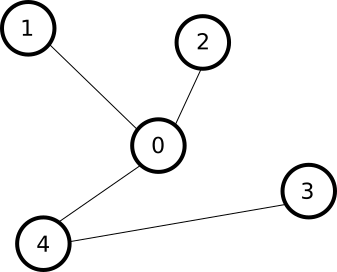
\includegraphics[width=0.3\textwidth]{sample.png}
  \caption{Illustration of the example}
\end{figure}

The following 4 pairs have a single road between them: $(0, 1), (0, 2), (0, 4), (3, 4)$.

The following 4 pairs have two roads between them: $(0, 3), (1, 2), (1, 4), (2, 4)$.

The following 2 pairs have three roads between them: $(1, 3), (2, 3)$.

This means that if for $K = 1, 2, 3$, the answers would be $4, 4, 2$ respectively.

\section*{Task}
Your task is to compute how many pairs of cities have exactly $K$ roads between them. You will implement the function \texttt{paths(N, K, F, T)}.
\begin{itemize}
  \item \texttt{paths(N, K, F, T)} - this function will be called exactly once by the judge.
  \begin{itemize}
    \item \texttt{N}: the number of cities in the kingdom.
    \item \texttt{K}: the number of roads between pairs of cities we are interested in.
    \item \texttt{F}: an array with $N - 1$ elements. \texttt{F[i]} ($0 \le i < N$) contains one of the cities that the $i$:th road connects.
    \item \texttt{T}: an array with $N - 1$ elements. \texttt{T[i]} ($0 \le i < N$) contains the other city that the $i$:th road connects.
    \item It is always possible to travel between any pair of cities using the roads.
    \item The function should return the number of pairs of cities that has exactly $K$ roads between them.
  \end{itemize}
\end{itemize}

\section*{Subtasks}
The problem consists of a number of subtasks. Each subtask gives some amount of points, and to pass
the subtask you must pass all the test cases in the subtask.

\begin{tabular}{|l|l|l|}
  \hline
  \textbf{Subtask} & \textbf{Points} & \textbf{Limits} \\ \hline
  1 & 9 & $1 \le K \le N \le 100$ \\ \hline
  2 & 19 & $1 \le K \le N \le 1\,000$ \\ \hline
  3 & 34 & $1 \le K \le 10$, $N \le 100\,000$ \\ \hline
  4 & 38 & $1 \le K \le N \le 100\,000$ \\ \hline
\end{tabular}

\section*{Input format}
The sample judge reads input in the following format:

\begin{itemize}
  \item line $1$: \texttt{N K}
  \item line $2$: \texttt{F[0] F[1] .. F[N - 2]}
  \item line $3$: \texttt{T[0] T[1] .. T[N - 2]}
\end{itemize}

\section*{Output format}
The sample judge will write a single line with the return value of \texttt{paths(N, K, F, T)}.
